\documentclass[tikz,border=8pt]{standalone}

\usepackage[T1]{fontenc}
\usepackage[utf8]{inputenc}
\usepackage{tikz}
\usetikzlibrary{arrows.meta,positioning}

\begin{document}
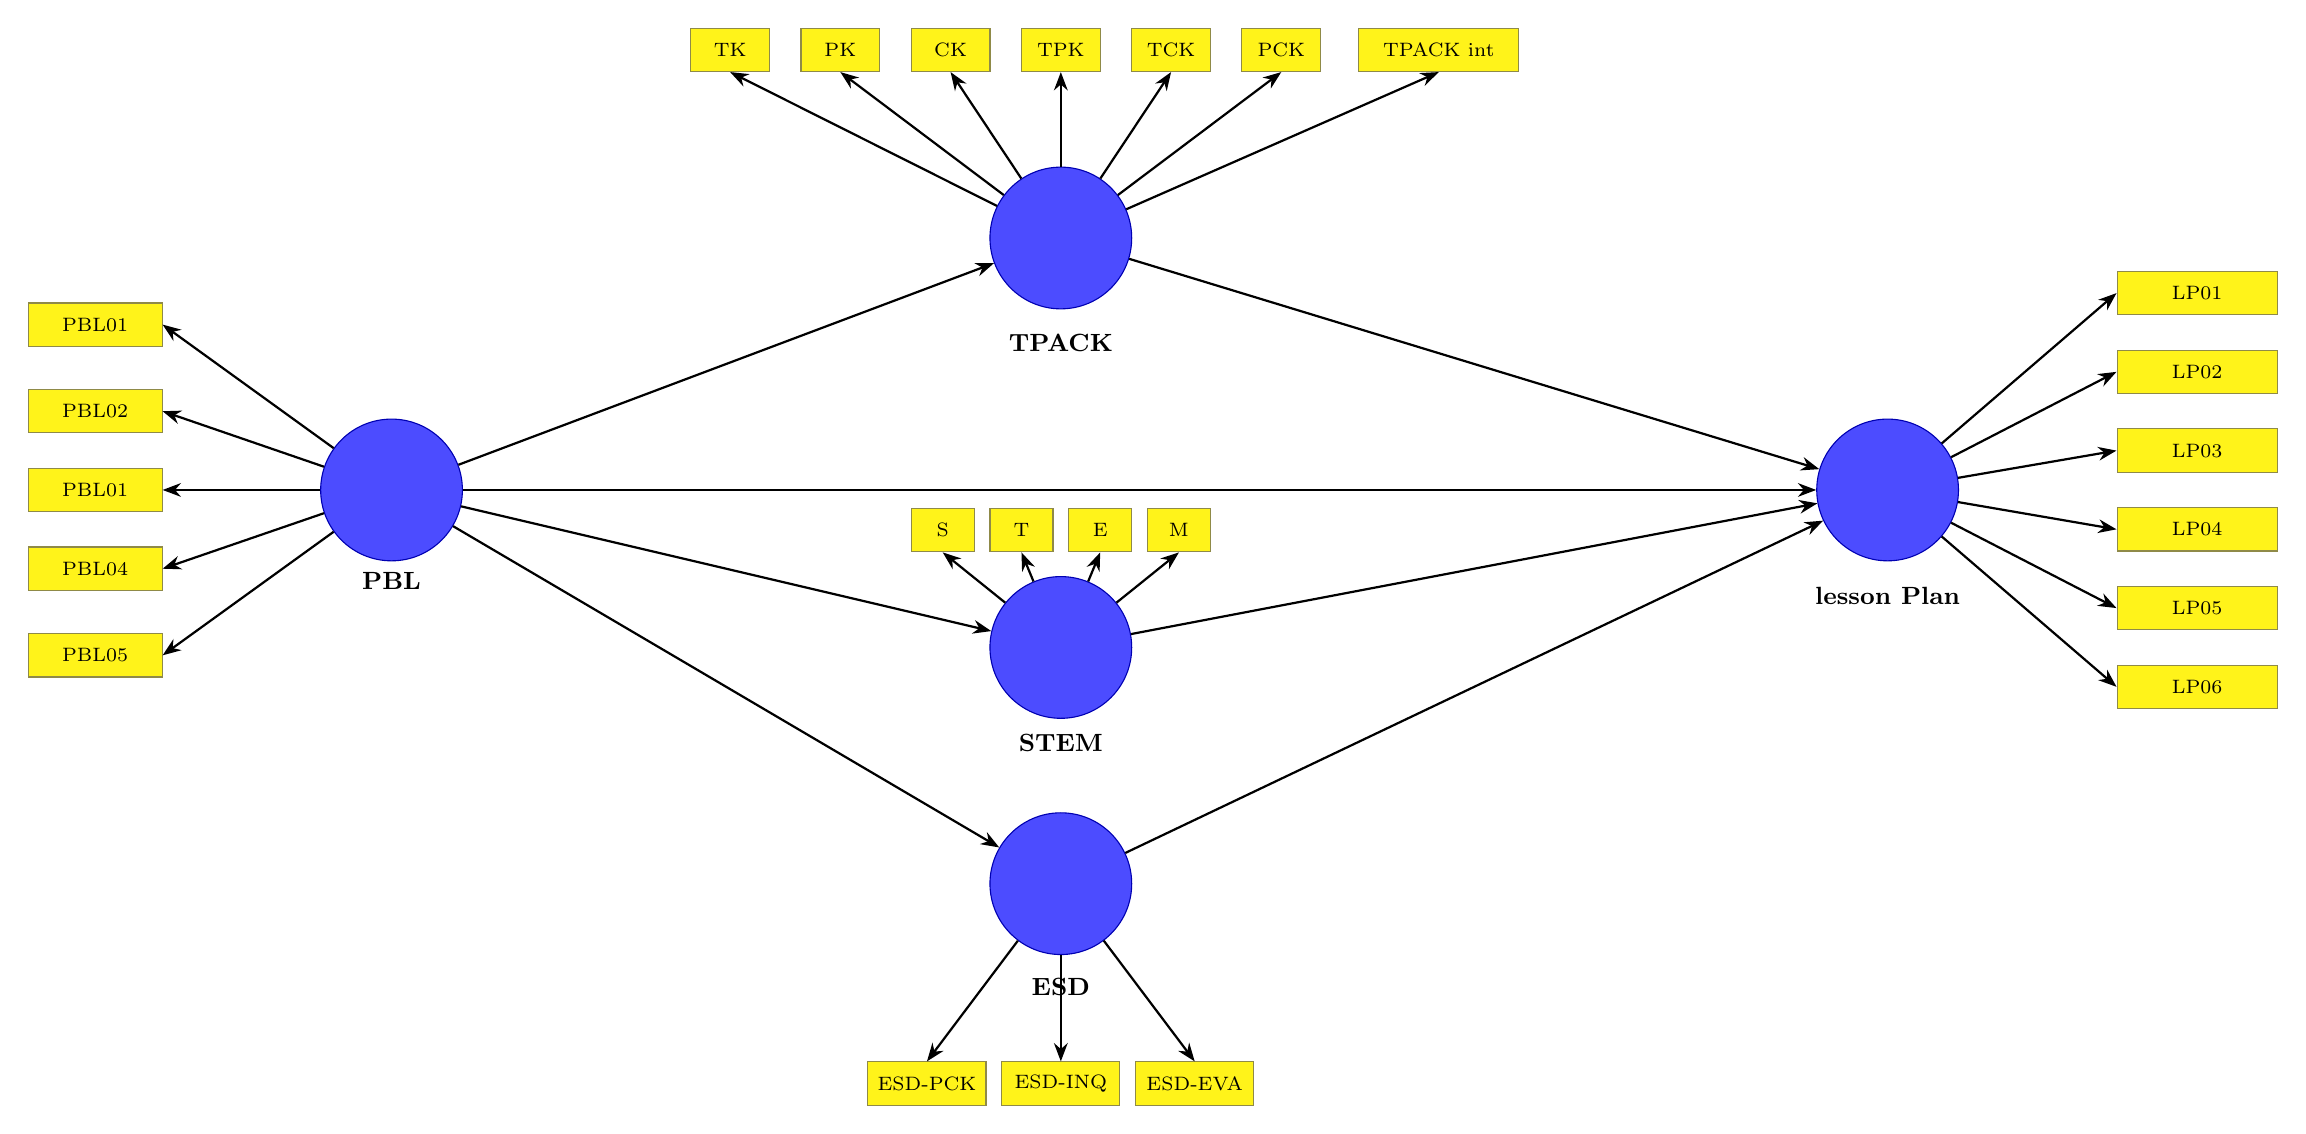
\begin{tikzpicture}[
  >=Stealth,
  line/.style={-Stealth,thick,draw=black},
  latent/.style={circle,draw=blue!70!black,fill=blue!70,minimum size=18mm,inner sep=0pt},
  llabel/.style={font=\small\bfseries,inner sep=1pt},
  ind/.style={rectangle,draw=yellow!50!black,fill=yellow!90,minimum width=17mm,minimum height=5.5mm,font=\scriptsize,align=center},
  indr/.style={ind,text width=18mm},
  indtop/.style={ind,minimum width=10mm},
  indstem/.style={ind,minimum width=8mm},
  indesd/.style={ind,minimum width=15mm}
]

% Latent nodes
\node[latent] (pbl) at (0,0) {};
\node[latent] (tpack) at (8.5,3.2) {};
% NOTE: STEM diturunkan lagi sesuai permintaan
\node[latent] (stem) at (8.5,-2) {};
% NOTE: ESD diturunkan lebih jauh agar tidak bertabrakan dengan STEM
\node[latent] (esd) at (8.5,-5) {};
\node[latent] (rpp) at (19.0,0) {};

\node[llabel,below=1mm of pbl] {PBL};
% NOTE: label TPACK diturunkan sedikit agar selalu terlihat jelas
\node[llabel,below=2.7mm of tpack] {TPACK};
\node[llabel,below=1.5mm of stem] {STEM};
% NOTE: label ESD diturunkan agar tidak menempel ke lingkaran
\node[llabel,below=2.6mm of esd] {ESD};
% NOTE: label lesson plan diturunkan agar lebih lega dari node kanan
\node[llabel,below=2.8mm of rpp] {lesson Plan};

% Structural paths
\draw[line] (pbl) -- (tpack);
\draw[line] (pbl) -- (stem);
\draw[line] (pbl) -- (esd);
\draw[line] (pbl) -- (rpp);
\draw[line] (tpack) -- (rpp);
\draw[line] (stem) -- (rpp);
\draw[line] (esd) -- (rpp);

% PBL indicators (left)
\node[ind,left=2.0cm of pbl,yshift=2.1cm] (pj1) {PBL01};
\node[ind,left=2.0cm of pbl,yshift=1.0cm] (pj2) {PBL02};
\node[ind,left=2.0cm of pbl] (pj3) {PBL01};
\node[ind,left=2.0cm of pbl,yshift=-1.0cm] (pj4) {PBL04};
\node[ind,left=2.0cm of pbl,yshift=-2.1cm] (pj5) {PBL05};
\draw[line] (pbl) -- (pj1.east);
\draw[line] (pbl) -- (pj2.east);
\draw[line] (pbl) -- (pj3.east);
\draw[line] (pbl) -- (pj4.east);
\draw[line] (pbl) -- (pj5.east);

% TPACK indicators (top)
% NOTE: jarak antar kotak atas diperlebar agar tidak saling menempel
\node[indtop,above=1.2cm of tpack,xshift=-4.2cm] (tk) {TK};
\node[indtop,above=1.2cm of tpack,xshift=-2.8cm] (pk) {PK};
\node[indtop,above=1.2cm of tpack,xshift=-1.4cm] (ck) {CK};
\node[indtop,above=1.2cm of tpack,xshift=0.0cm] (tpk) {TPK};
\node[indtop,above=1.2cm of tpack,xshift=1.4cm] (tck) {TCK};
\node[indtop,above=1.2cm of tpack,xshift=2.8cm] (pck) {PCK};
\node[indtop,above=1.2cm of tpack,xshift=4.8cm,text width=18mm] (tpackint) {TPACK int};
\draw[line] (tpack) -- (tk.south);
\draw[line] (tpack) -- (pk.south);
\draw[line] (tpack) -- (ck.south);
\draw[line] (tpack) -- (tpk.south);
\draw[line] (tpack) -- (tck.south);
\draw[line] (tpack) -- (pck.south);
\draw[line] (tpack) -- (tpackint.south);

% NOTE (PANAH STEM -> S/T/E/M):
% - Parameter `above=... of stem` mengatur JARAK VERTIKAL box S/T/E/M dari node STEM.
% - Semakin kecil nilainya, semakin pendek panah dari STEM ke box indikator.
% - Contoh: 1.35cm -> 1.00cm untuk memendekkan panah.
% - Parameter `xshift` mengatur sebaran kiri-kanan. Nilai yang lebih kecil (mis. +/-1.2)
%   juga membuat panah diagonal lebih pendek.
\node[indstem,above=0.3cm of stem,xshift=-1.5cm] (s) {S};
\node[indstem,above=0.3cm of stem,xshift=-0.5cm] (t) {T};
\node[indstem,above=0.3cm of stem,xshift=0.5cm] (e) {E};
\node[indstem,above=0.3cm of stem,xshift=1.5cm] (m) {M};
% NOTE: baris berikut adalah garis panah STEM -> masing-masing indikator
\draw[line] (stem) -- (s.south);
\draw[line] (stem) -- (t.south);
\draw[line] (stem) -- (e.south);
\draw[line] (stem) -- (m.south);

% ESD indicators (below esd)
\node[indesd,below=1.35cm of esd,xshift=-1.7cm] (esd1) {ESD-PCK};
\node[indesd,below=1.35cm of esd] (esd2) {ESD-INQ};
\node[indesd,below=1.35cm of esd,xshift=1.7cm] (esd3) {ESD-EVA};
\draw[line] (esd) -- (esd1.north);
\draw[line] (esd) -- (esd2.north);
\draw[line] (esd) -- (esd3.north);

% lesson plan (RPP) indicators (right)
% NOTE: style 'indr' memastikan lebar box kanan konsisten
\node[indr,right=2.0cm of rpp,yshift=2.5cm] (r1) {LP01};
\node[indr,right=2.0cm of rpp,yshift=1.5cm] (r2) {LP02};
\node[indr,right=2.0cm of rpp,yshift=0.5cm] (r3) {LP03};
\node[indr,right=2.0cm of rpp,yshift=-0.5cm] (r4) {LP04};
\node[indr,right=2.0cm of rpp,yshift=-1.5cm] (r5) {LP05};
\node[indr,right=2.0cm of rpp,yshift=-2.5cm] (r6) {LP06};

\draw[line] (rpp) -- (r1.west);
\draw[line] (rpp) -- (r2.west);
\draw[line] (rpp) -- (r3.west);
\draw[line] (rpp) -- (r4.west);
\draw[line] (rpp) -- (r5.west);
\draw[line] (rpp) -- (r6.west);

\end{tikzpicture}
\end{document}
